\section{Satisfiability modulo theories - SMT}
In computer science and mathematical logic, the \textbf{SMT} problem is a decision problem for logical formulas with respect to combinations of background theories expressed in \textbf{FOL}.\\
SMT can be thought of as a form of the constraint satisfaction problem and thus a certain formalized approach to constraint programming. \\

\subsection{SMT implementation}
To implement models in \textbf{SMT} we will use the library \textbf{Z3} in python notebooks.
\subsubsection{Without rotation}
To implement the model described in \hyperref[subsubsec:base-without-rot]{model without rotation} we used as variables: 
\begin{itemize}
    \item \textbf{x} to represent the X coordinates of the circuit;
    \item \textbf{y} to represent the Y coordinates of the circuit;
    \item \textbf{Height} to represent the maximum height reached by the circuits;
\end{itemize}
And as parameters we have:
\begin{itemize}
    \item \textbf{$N$} which represent the number of circuit;
    \item \textbf{$S$} to represent the set of circuit from 0\dots N;
    \item \textbf{$w_i$} to represent the width of circuit i;
    \item \textbf{$h_i$} to represent the height of circuit i;
    \item \textbf{WIDTH} which represent the width of the plate;
\end{itemize}
Then we added to the solver the following conditions: 
\begin{align}
    &width\_boundaries \equiv \forall{i \in  S}.(x_i \geq 0  \wedge  x_i + w_i \leq \textit{WIDTH}),\\
    &height\_boundaries \equiv \forall{i \in  S}.(y_i \geq 0  \wedge  y_i + h_i \leq \textit{HEIGHT}),
\end{align}
\begin{align}
   & no\_overlap\_cons \equiv \forall (i, j \in  S \text{ where } i \neq j).(\\
    &( x_i + w_i \leq x_j) \: \lor \\
    &( x_i - w_j \geq x_j) \: \lor \\
    &( y_i + h_i \leq y_j) \: \lor \\
    &(y_i - h_j \geq y_j)).
\end{align}
Hence, as the conjunction of all constraints we'll have: 
\begin{align}
    all\_constraints \equiv width\_boundaries \wedge height\_boundaries \wedge no\_overlap\_cons
\end{align}
Finally, by minimizing the \textbf{HEIGHT} we are reducing the empty area created by placing the circuits in the plate as the sum of area of the circuit is constant, although the \textbf{WIDTH} is fixed. 

\subsubsection{With rotation}
For the version of the model considering also the rotation, based on the previous model, we added a list of binary variables, which domain is defined as: 
\begin{equation}
    rot\_domain \equiv \forall{i \in S}.( rot_i \geq 0 \wedge  rot_i \leq 1)
\end{equation}
And we are considering the fact that: 
\begin{itemize}
    \item $rot_i$ is equal to 0, then the circuit $i$ is not rotated;
    \item $rot_i$ is equal to 1, then circuit $i$ is rotated by 90$^{\circ}$;
\end{itemize}
Then, we slightly modified constraints of the no rotation version as follows: 
\begin{align}
   & width\_boundaries \equiv \forall{i \in  S}.(x_i \geq 0  \wedge  x_i +(1-rot_i) w_i+ rot_i h_i \leq \textit{WIDTH})\\
    &height\_boundaries \equiv \forall{i \in  S}.(y_i \geq 0  \wedge  y_i + (1-rot_i)h_i + rot_i w_i \leq \textit{HEIGHT})
\end{align}
We simply considered that if a certain circuit $i$ is rotated, the $w_i$ and $h_i$ will be exchanged, so to compute the coordinates of the opposite corner, we will have to do the same.
\begin{align}
    &no\_overlap\_cons \equiv \forall (i, j \in  S \text{ where } i \neq j).(\\
      &(x_i + rot_i * h_i + (1 - rot_i) * w_i <= x_j) \: \\
     &\lor(y_i + rot_i * w_i + (1 - rot_i) * h_i <= y_j) \: \\
     &\lor(x_i - rot_j * h_j - (1 - rot_j) * w_j >= x_j) \: \\
     &\lor(y_i - rot_j * w_j - (1 - rot_j) * h_j >= y_j)\:
\end{align}
Also in this model, we set a objective function, the $height$, and our aim is to minimize it.

\subsection{Symmetry breaking}\label{subsec:smt-symmetry-breaking}
There are two symmetry breaking conditions, the first one is composed by the following:
\begin{equation}
    x_{big} * 2 \leq width \wedge y_{big}* 2\leq height
\end{equation}
In this case, we are forcing the biggest circuit to be placed in the a quadrant of the plate: 
\begin{figure}[!h]
 \centering
 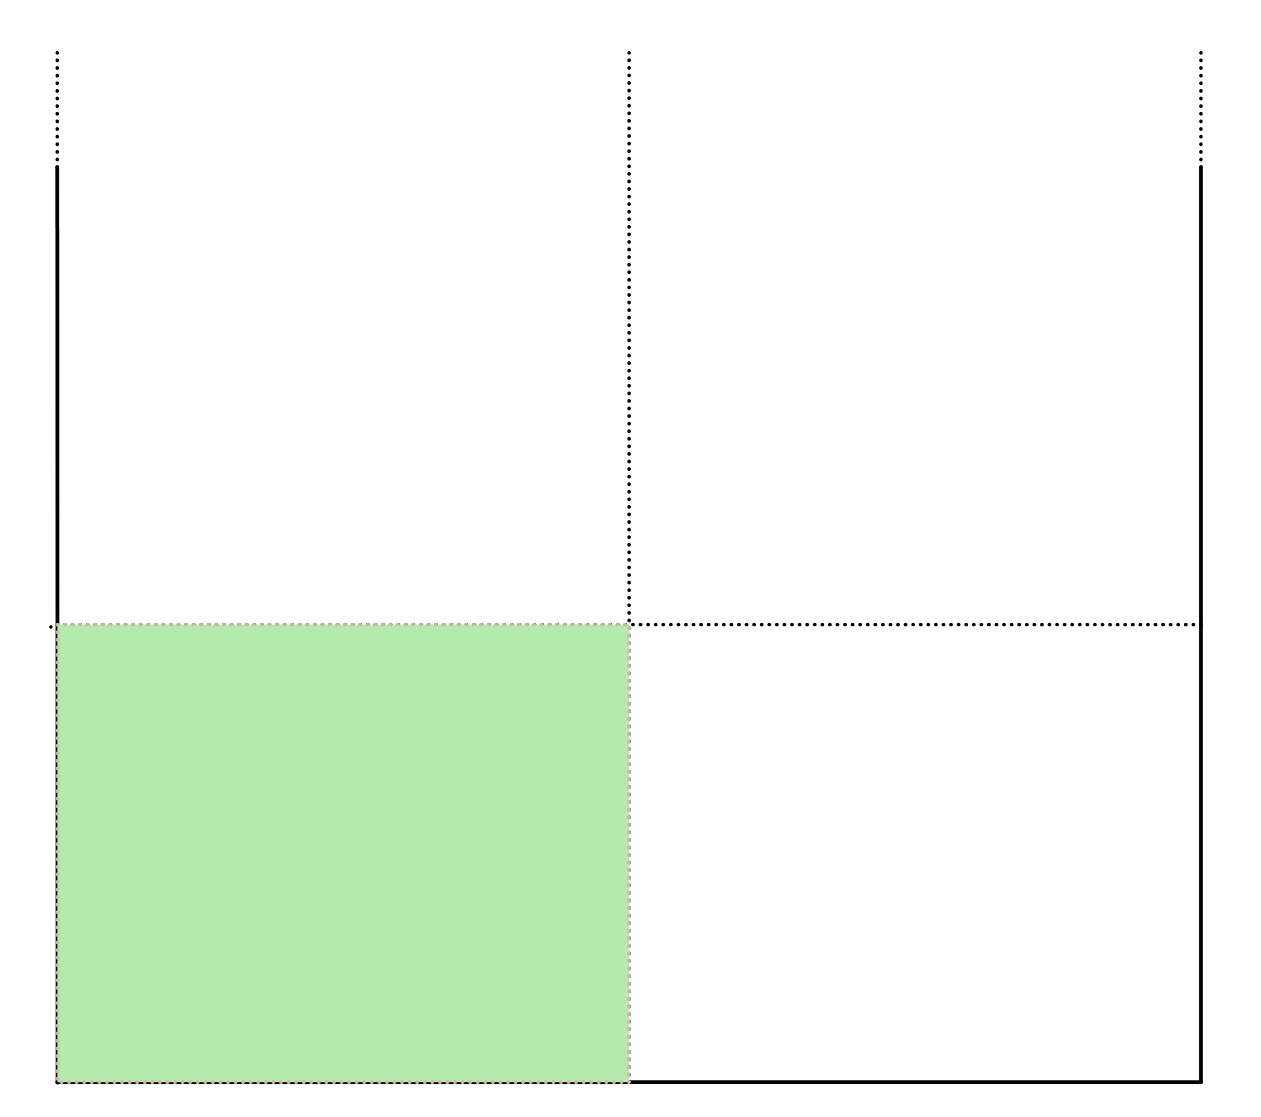
\includegraphics[width=12cm, height=8cm]{images/quadtants.PNG}
 \caption{Green area is the possible position of the biggest circuit}
\end{figure}\\
Meanwhile, the second one is the extreme case of the previous one, because we are imposing these conditions:
\begin{equation}
    x_{big} == 0 \wedge y_{big} == 0
\end{equation}
where $biggest$ is the index of the circuit with the biggest area. And in this case, the biggest circuit will be placed in the lower-left corner of the plate. Differently from what has been done with the MiniZinc implementation, here both of the symmetry constraints will be kept since the extreme case seems to perform better overall.  

\subsection{SMT models comparisons}
Now, we are going show the performance of different models over the 40 instances: \\
\begin{table}[!h]
    \begin{tabular}{|c| p{2cm} | p{2 cm} | p{1.5cm} | p{3.5cm} | c |}\hline
        Model &Rotation& Symmetry breaking& Solved instance & Mean time( solved instances) (s) & total time (s) \\\hline
           A &No  & No  & 22  & 16.78 & 369.11 \\ \hline
           B &No  & Yes & 24  & 29.51 & 708.27 \\ \hline
           C &Yes & No  & 14  & 38.94 & 545.23 \\ \hline
           D &Yes & Yes & 14  & 60.00 & 840.03 \\ \hline
    \end{tabular}
    \caption{SMT model performances}
    \label{tab:smt-performance}
\end{table}
\\
We can notice from the table that the model B has solved two instances in more w.r.t. the model A (instance 19 and 28 respectively with 242.95s and 180.94s), and because of this, it's mean time is higher than the one of A. 
\subsubsection{No rotation vs rotation}

From the previous table, we can notice a clearly improvement of the performance between model without rotation and the one with rotation, this is because in the latter one we have to consider when pieces are rotated, and the combination is $2^N$ times in more w.r.t. first one. 
\subsubsection{Two cases of symmetry breaking}

As we said in the \hyperref[subsec:smt-symmetry-breaking]{\S 4.2} there are two cases of symmetry breaking, the following table shows the different of performance when executing the models for instances from 10 to 19 as they are those more difficult to solve. We will only consider the model with rotation.

% Please add the following required packages to your document preamble:
% \usepackage[table,xcdraw]{xcolor}
% \documentclass[xcolor=table]{beamer}
% If you use beamer only pass "xcolor=table" option, i.e. 
\begin{table}[!h]
    \centering
    \begin{tabular}{|l|l|l|}
        \hline
         & Normal case & Extreme Case \\ \hline
        Instances 10 & 149.46      & 108.86       \\ \hline
        Instances 11 & 0.00         & 0.00          \\ \hline
        Instances 12 & 6.18        & 29.22        \\ \hline
        Instances 13 & 151.64      & 101.55       \\ \hline
        Instances 14 & 0.00         & 162.97       \\ \hline
        Instances 15 & 17.47       & 130.00       \\ \hline
        Instances 16 & 0.00         & 0.00          \\ \hline
        Instances 17 & 227.20      & 46.30        \\ \hline
        Instances 18 & 0.00         & 250.02       \\ \hline
        Instances 19 & 0.00         & 0.00          \\ \hline
        Solved instances & 5           & 7            \\ \hline
        Mean (All instances) & 205.1956    & 172.8912     \\ \hline
        Mean (Solved instances) & 110.40    & 118.42     \\ \hline
        Total time       & 2051.956    & 1728.912     \\ \hline
    \end{tabular}
    \caption{Execution statistics of instances 10 to 19.}
    \label{tab:my-table}
\end{table}
For the instances which are not solved within 300s, we abort the execution and consider the execution time as 0s. \\
The extreme case can solve 2 more instances w.r.t. the normal one, and if we recompute the mean time for extreme case, considering only instances solved by the normal case, the result would be \emph{83.19}, which is much lower than the normal case. 

\begin{figure}[!h]
 \centering
 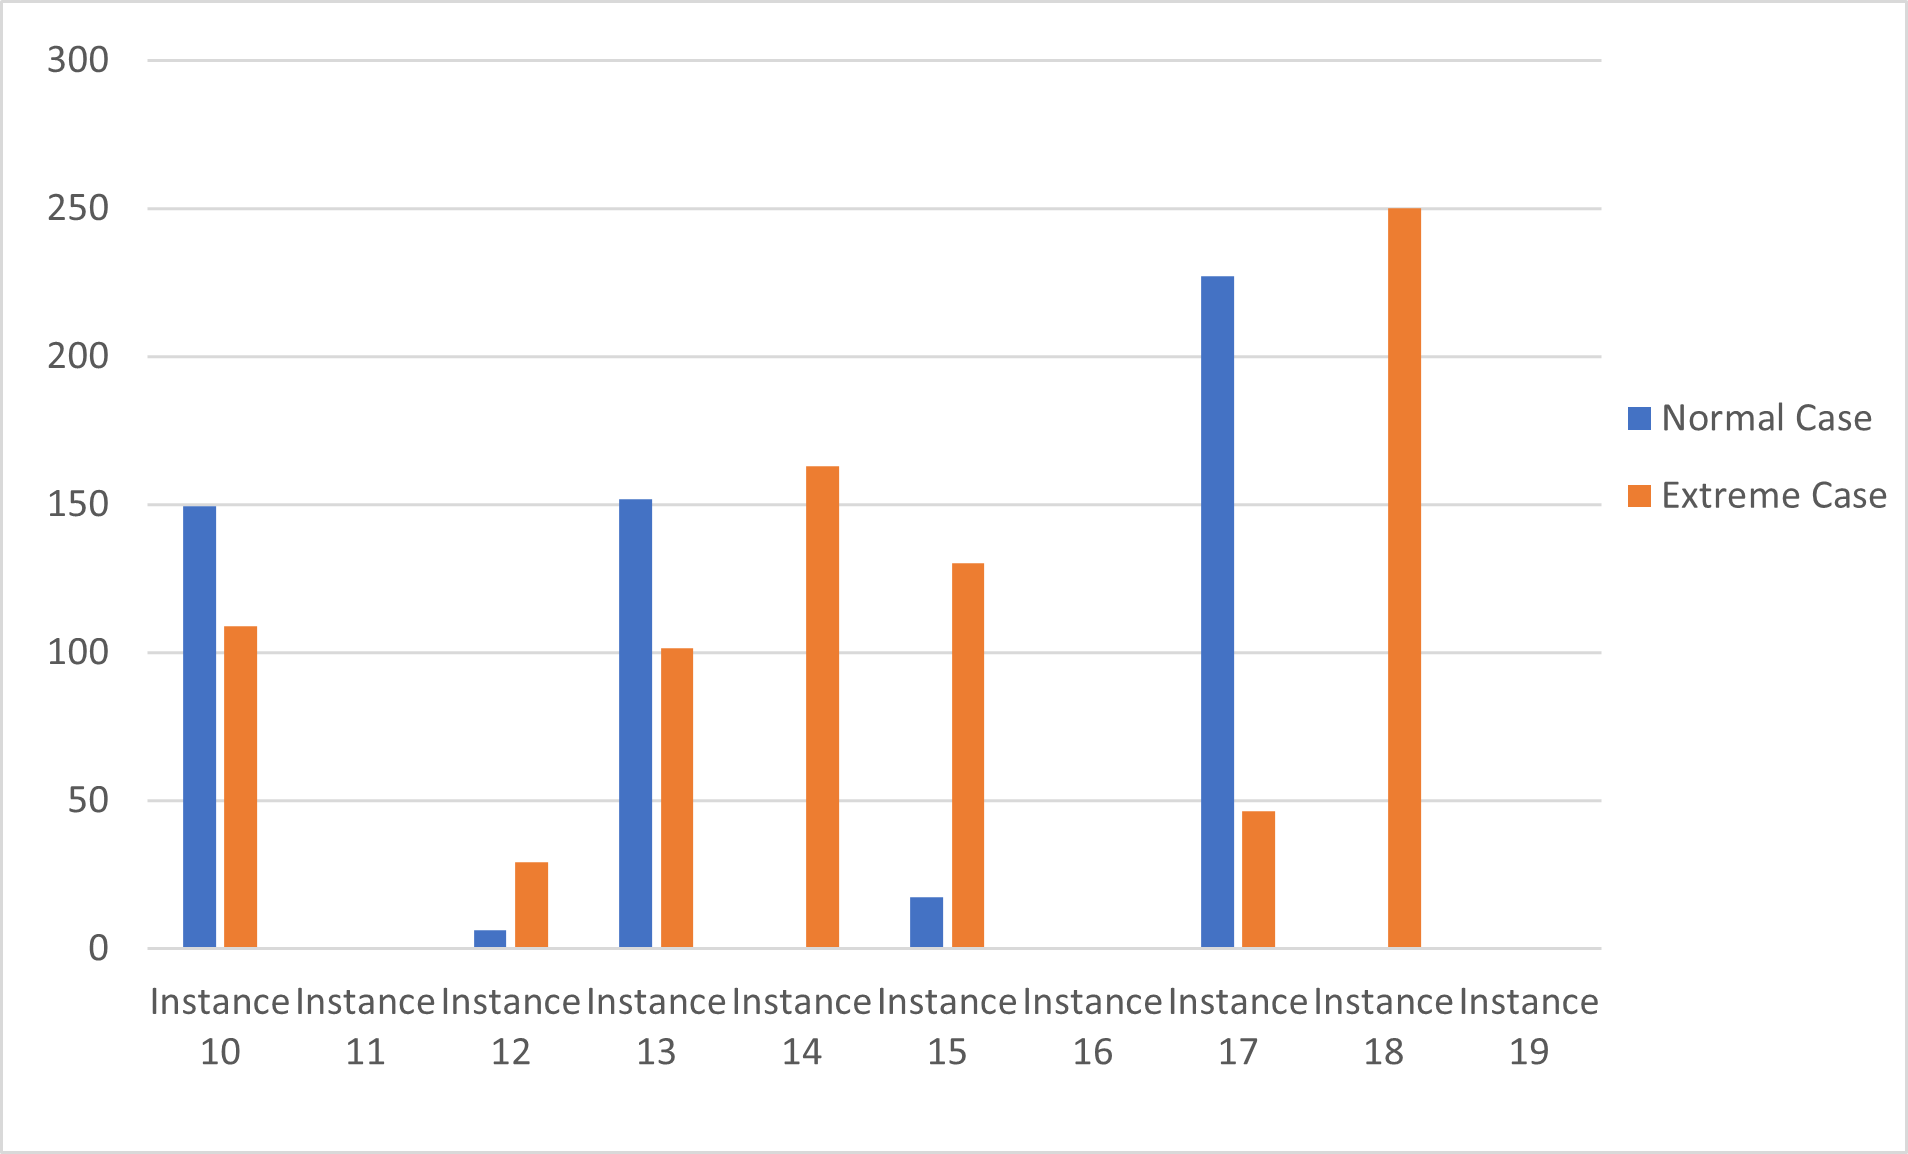
\includegraphics[width=14cm, height=10cm]{images/sym_breaking_smt_comparison.png}
 \caption{Symmetry breaking comparison.}
 \label{fig:sym-breaking-comparison}
\end{figure}

What we can see from the \hyperref[fig:sym-breaking-comparison]{graph} is that the extreme case works better.\\

Differently from the \textbf{CSP}, we can see a improvement of the performance of the extreme case of symmetry breaking. 

\clearpage